\chapter{Methodology}%
Construction of associative memory using \Snn\cite{base} in this method consist of four phases
\begin{enumerate}
    \itemsep 0em
    \item Initialization : Initialization of \Snn and the input spiking signals
    \item Structure formation : New connection with neighboring neuron are formed
    \item Parameter training : Optimize weight of synapse based on STDP
    \item Pruning : Removing unnecessary connection to improve efficiency
\end{enumerate}
\section{Initialization}
It involves two sub process in which the data is preprocessed and converted
into spiking signals and the network is initialized
\subsection{Initialization input spiking signals}
The input to the SNN are spiking signals for that the input values need to be
converted into spiking signals. For the example purpose here MNIST dataset is
used which contains handwritten characters on digits. The figure
\ref{preprocessing} show the steps involved

\begin{figure}[h!]
    \centering
    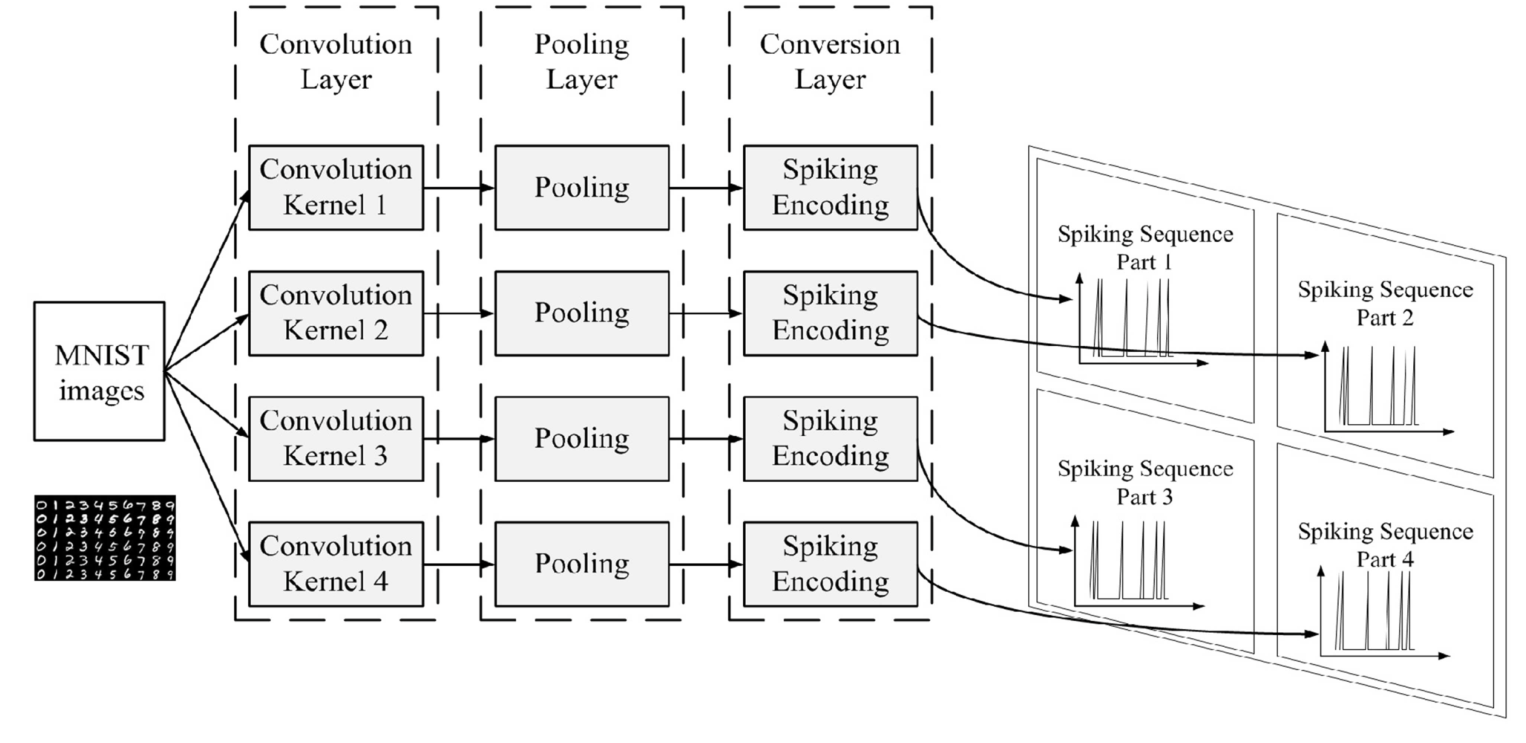
\includegraphics[width=0.7\linewidth]{preprocessing}
    \caption{Data preprocessing}
    \label{preprocessing}
\end{figure}

Four convolutional kernels of size $4X4$ shown in \ref{kernel} is used to
extract the features from the image pixel values. The input image into the
kernel is of size $28X28$ and the convolutional kernels reduce the shape into
$24X24$. Next these values are passed through a max pooling layer of size
$2X2$. It reduces the size of image to $12X12$. The conversion layer convert
these values into the spiking encoding.Pixel value in the range of [0,255]
converted to delay in spike from [0,100]ms. The higher the value, shorter the
delay.
\begin{figure}[h!]
    \centering
    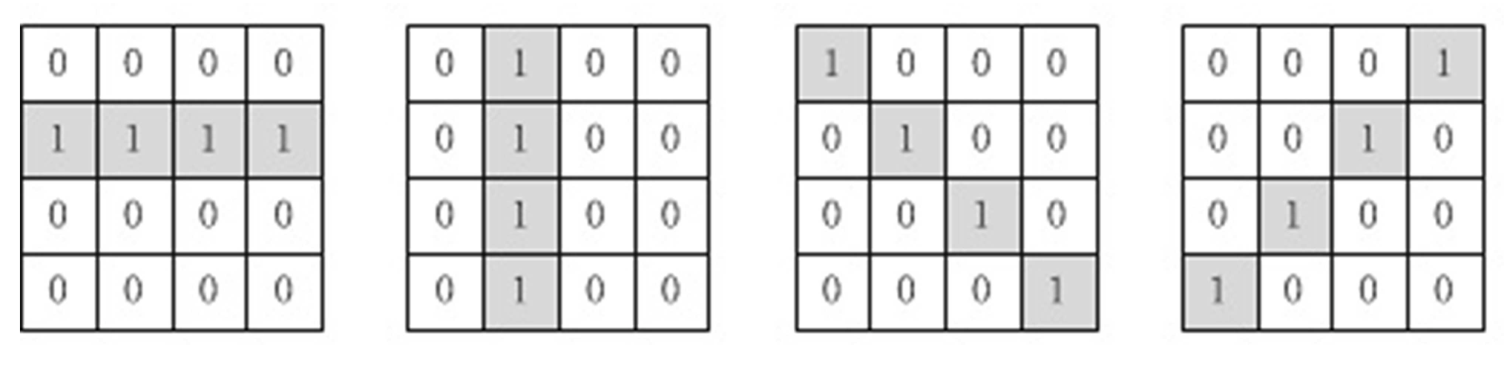
\includegraphics[width=0.7\linewidth]{kernels}
    \caption{Kernels used}
    \label{kernel}
\end{figure}
In order to cover the values first min-max normalization is used in which if
the value of a pixel is d then,
\begin{equation*}
    R(d)=\frac{d-d_{min}}{d_{max}-d_{min}}
\end{equation*}

Where d{min} and d{max} are maximum and minimum pixel values. Power encoding is
used to get the spike time of pixel d,
\begin{equation*}
    S(d)=(R(d)-1)^2 \times (T_{max}-T_{min})+T{min}
\end{equation*}
where T{min} and T{max} are starting and stopping time of spike.
\subsection{Initialization of \Snn}
The memory \nn in this method consists of three layers input, memory and output
as shown in figure \ref{structure}. The spiking signal input is fed into the
input layer. For the neuron, the LIF model is used. The memory layer grows new
connections to remember them. The output layer is responsible for generating
the output. The number of neurons in both the input and memory layers is the
same as the number of input spiking signals which is 576. The output layer
consists of 10 neurons which are equal to the number of output classes.
\begin{figure}[h!]
    \centering
    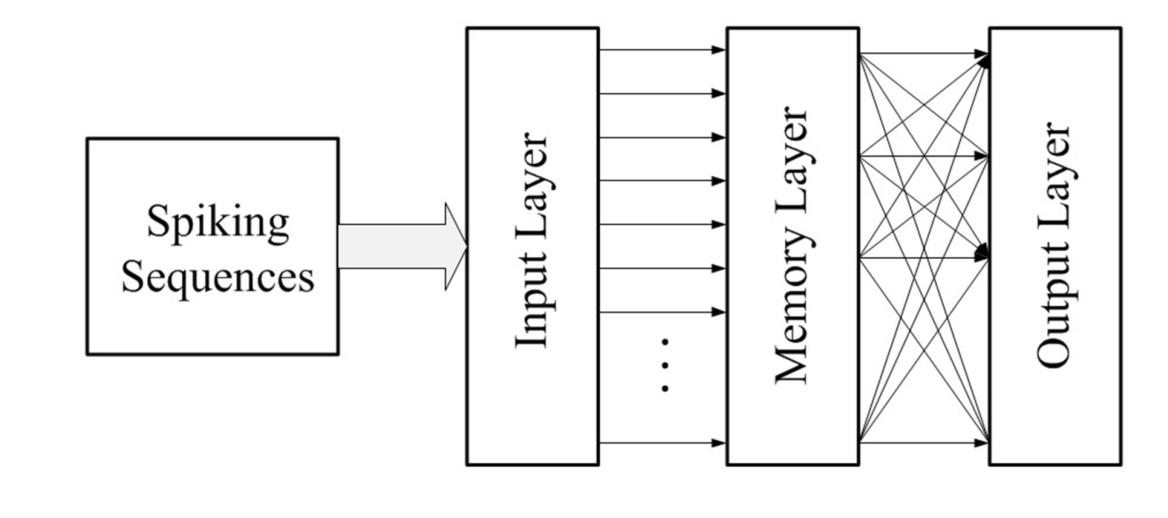
\includegraphics[width=0.7\linewidth]{structure}
    \caption{Structure of network}
    \label{structure}
\end{figure}

The connection from the input layer to the memory layer is one-to-one style.
The weight of the synapse is set to 50 as an initial value. It helps in
provoking enough response in the memory layer based on Hebb's learning
rule\cite{hebbs} to take place.

Each neuron in layers is assigned a coordinate value. By using a spatial to
temporal mechanism which encodes the spatial information of pixel values into
delay of connection from the input layer to the memory layer as shown in the
figure \ref{delay}. The delay of a connection from a neuron i(x,y) where x and
y are coordinates of the pixel values in a $p \times q$ input layer to
corresponding neuron in the memory layer is calculated as
\begin{equation*}
    delay_{im(x,y)}=x*p+y+1
\end{equation*}
\begin{figure}[h!]
    \centering
    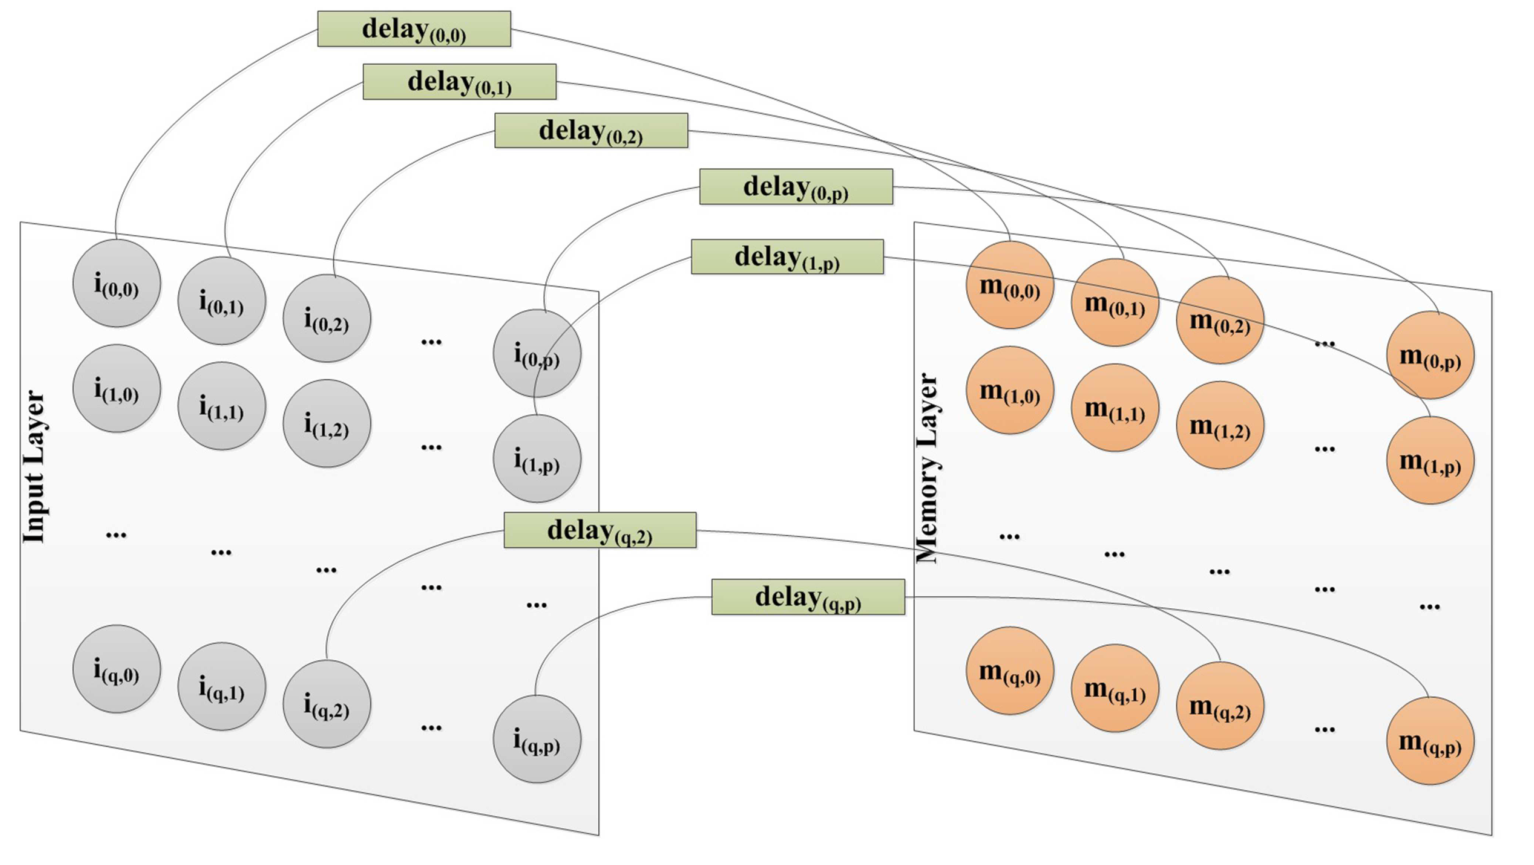
\includegraphics[width=0.7\linewidth]{delay}
    \caption{Delay for neuron}
    \label{delay}
\end{figure}
\section{Structure formation}
During the structure formation phase are fed into the network. The behaviour of
neurons in the memory layer is recorded and new connections are made within the
memory layer based on Hebb's learning rule\cite{hebbs}. New connection
conditions are based on their threshold values of distance and time difference
in firing two neurons to avoid explosive growth of connections. If there are
two neurons which satisfy the threshold conditions on delay and distance in
firing and there is no connection between them a new connection is established
between them.The smaller the threshold lesser the number of connections that
will be created.

It is repeated until the stopping condition is satisfied. Due to the leaking
characteristics of the LIF model used the connection from the memory layer to
output layer implements a spatial-to-temporal mechanism discussed earlier is
used. The delay of connection from the memory layer to the output layer is
calculated as
\begin{equation*}
    delay_{mo(x,y)}=[N_m-delay_{im(x,y)}]+1
\end{equation*}
\section{Parameter training}
This phase is based on the ideas of STDP and reinforcement learning. This phase
checks the recall ability of the network for the set of inputs. This phase does
not change the weights of the connection between layers but rather changes the
weight of the connection within the memory layer itself. For this process when
a spiking sequence is fed into the network the most frequently fired neuron in
the output layer is considered as output. If the network could correctly recall
then no optimization need to be done else the weights need to be adjusted. It
works based on the following algorithm \\Step 1:Pick an input image\\ Step
2:Feed input to the network\\ Step 3:Pick If the result of the output layer is
correct go to 1 else 4\\ Step 4:Identify incorrectly firing set of neurons in
output layer $S_{O}$ memory layer $S_{M}$ \\ Step 5:If i is a neuron in $S_M$
and and j is a neuron in $S_O$ and weight of connection between them is
$W_{i,j}$, then $W_{i,j}=W_{i,j}*Shrink\_Coeff$\\ This process repeated for all
the images.The value of $Shrink\_Coeff$ is constant between 0 and 1.figure
\ref{recall} shows the firing behavior of the memory layer when it is supplied
with an input image corresponding to the number six. Colours indicate the time
at which the spike occurred and lines indicate the connection between neurons.
\begin{figure}[h!]
    \centering
    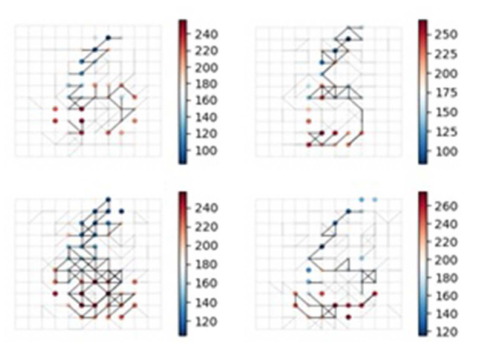
\includegraphics[width=0.7\linewidth]{recall}
    \caption{Recall response for number 6}
    \label{recall}
\end{figure}
\section{Pruning}
This phase help in improving the efficiency of the network. In this phase if
the weight of a connection is less than the threshold (here 3), connection will
be removed. Also, if there is a neuron in memory layer in memory layer which
does not have any connections to output layer, the connection from input layer
to that neuron will also be deleted.
% This section describes the research methods used in the seminar, including the
% participants, data collection techniques, and data analysis methods.